\documentclass[12pt]{article}
\usepackage[papersize={8cm,12cm},margin={.5cm,.5cm}]{geometry}
\usepackage{common}
\usepackage{xeCJKfntef}
\usepackage{graphicx}
\makeatletter
\DeclareFontFamily{U}{tipa}{}
\DeclareFontShape{U}{tipa}{m}{n}{<->tipa10}{}
\newcommand{\arc@char}{{\usefont{U}{tipa}{m}{n}\symbol{62}}}%
\newcommand{\arc}[1]{\mathpalette\arc@arc{#1}}
\newcommand{\arc@arc}[2]{\sbox0{$\m@th#1#2$}%
  \vbox{
    \hbox{\resizebox{\wd0}{\height}{\arc@char}}
    \nointerlineskip
    \box0
  }%
}
\makeatother
\begin{document}
\begin{problem}
\item[3.] 有一直徑為 $\overline{AB}$ 的圓,圓上有 $C$、$D$、$E$、$F$ 四點,如圖(三)所示。已知 $\overline{AB} = 10$,$\overline{AC} = 6$,$\overline{AD} = 8$,$\overline{AE} = 5$,$\overline{AF} = 9$,則下列\CJKunderdblline*{弧長}關係何者正確?
  \begin{figure}[ht]
    \centering
    \vspace*{-1ex}
    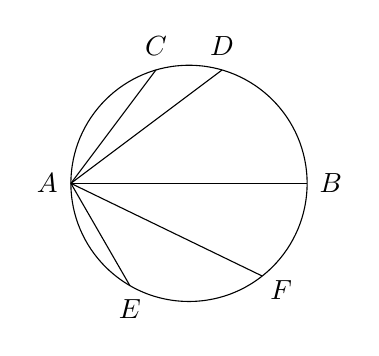
\begin{tikzpicture}
      \draw (0,0) circle (1.5cm);
      \draw (-1.5,0) -- (1.5,0);
      \draw (-1.5,0) -- (-.42,1.44);
      \draw (-1.5,0) -- (.42,1.44);
      \draw (-1.5,0) -- (-.75,-1.3);
      \draw (-1.5,0) -- (.93,-1.177);
      \node at (-1.8,0) {$A$};
      \node at (1.8,0) {$B$};
      \node at (-.42,1.74) {$C$};
      \node at (.42,1.74) {$D$};
      \node at (-.75,-1.6) {$E$};
      \node at (1.17,-1.357) {$F$};
    \end{tikzpicture}
    \vspace*{-1ex}
    \caption*{圖(三)}
    \vspace*{-2ex}
  \end{figure}
  \footnotesize
  \begin{choices}
    \item $\arc{AC} + \arc{AD} = \arc{AB}$,且 $\arc{AE} + \arc{AF} = \arc{AB}$
    \item $\arc{AC} + \arc{AD} = \arc{AB}$,且 $\arc{AE} + \arc{AF} \neq \arc{AB}$
    \item $\arc{AC} + \arc{AD} \neq \arc{AB}$,且 $\arc{AE} + \arc{AF} = \arc{AB}$
    \item $\arc{AC} + \arc{AD} \neq \arc{AB}$,且 $\arc{AE} + \arc{AF} \neq \arc{AB}$
  \end{choices}
\end{problem}
\end{document}
